\documentclass[]{article}
\usepackage{fullpage}
\usepackage{enumerate}
\usepackage[T1,T2A]{fontenc}
\usepackage[utf8]{inputenc}
\usepackage[bulgarian]{babel}
\usepackage{soul}
\usepackage{graphicx}

\usepackage{usecases}

%\renewcommand{\thesection}{\Roman{section}} 
%\renewcommand{\thesubsection}{\thesection.\Roman{subsection}}
\renewcommand{\thesubsection}{\arabic{subsection}.}

\begin{document}

\title{\sc{Информационна система на агенция за недвижими имоти}\\Част II: Модел на потребителските случаи}
\author{Екип $\pi \approx 3.1$}

\maketitle

\begin{center}

\begin{tabular}{r|l}
%\hline
71469	& Георги Димов \\ %\hline
71473	& Цветан Цветанов \\ %\hline
71488	& Антон Дудов \\ %\hline
71490	& Венцислав Конов \\ %\hline
71492	& Александър Танков \\ %\hline
71508	& Красимир Тренчев \\ %\hline
71512	& Александър Велин \\ %\hline
71524	& Анджелика Туджарска \\ %\hline
71529	& Александър Бранев \\ %\hline
855240	& Мартин Стоев \\ %\hline
\end{tabular}

\end{center}

\clearpage

%\tableofcontents
%\clearpage

\section*{Визия}

Трябва да се проектира информационна система за стартираща агенция за недвижими имоти.

Целта на информационната система е да осигури уеб интерфейс, чрез който брокери на агенцията да могат по-лесно да намират наематели и купувачи за имотите на своите клиенти. Връзката между продавачите и наемодателите с брокер ще се осъществява извън рамките на системата. Потребители на системата ще бъдат брокери, наематели и купувачи, администратор и одитор.

Създаването на новата информационна система цели да реши проблема с некоректното и неточно описание в обявите за имоти, което дават продавачи и наемодатели, като управлението на обявите ще се извършва от брокерите на агенцията. Системата ще позволява на брокерите да създават и редактират обяви за недвижими имоти, а на наематели и купувачи – да имат гъвкав и удобен интерфейс за търсене на обяви по различни критерии; да инициират комуникация с брокер и да дават своята оценка за обяви и брокери. Всяка обява и всеки брокер имат собствен рейтинг (по скала от 0 до 5), който е средна стойност спрямо всички гласове, подадени за съответната обява или брокер от регистрирани потребители. Рейтингът на брокера не се отразява на рейтинга на неговите обяви, и самите рейтинги имат само информационна стойност за потребителите на системата (т.е., не оказват влияние при търсене, преглед и т.н.).

Всички счетоводни и финансови процеси в агенцията не са предмет на информационната система.

Информационната система ще предоставя възможност за комуникация в реално време на потребителите с брокер на агенцията посредством обмяна на текстови съобщения между двете страни (т.н. "чат"), както и възможност потребителите да изпращат асинхронно текстови съобщения на брокерите (т.н. "контактна форма").

Системата трябва да поддържа одит лог, в който да записва всички действия на регистрирани потребители в системата. 
Записват се всички промени върху потребителските профили и обявите, както и изпратените съобщения от контакт формата.
В одит лога не отразяват промени, породени от рейтинговата система. Одит лога може да се чете само от одиторският акаунт, и не може да се променя от никого.

\clearpage

\section*{Use case модел} %FIXME

        \begin{figure}[h]
        \centering
        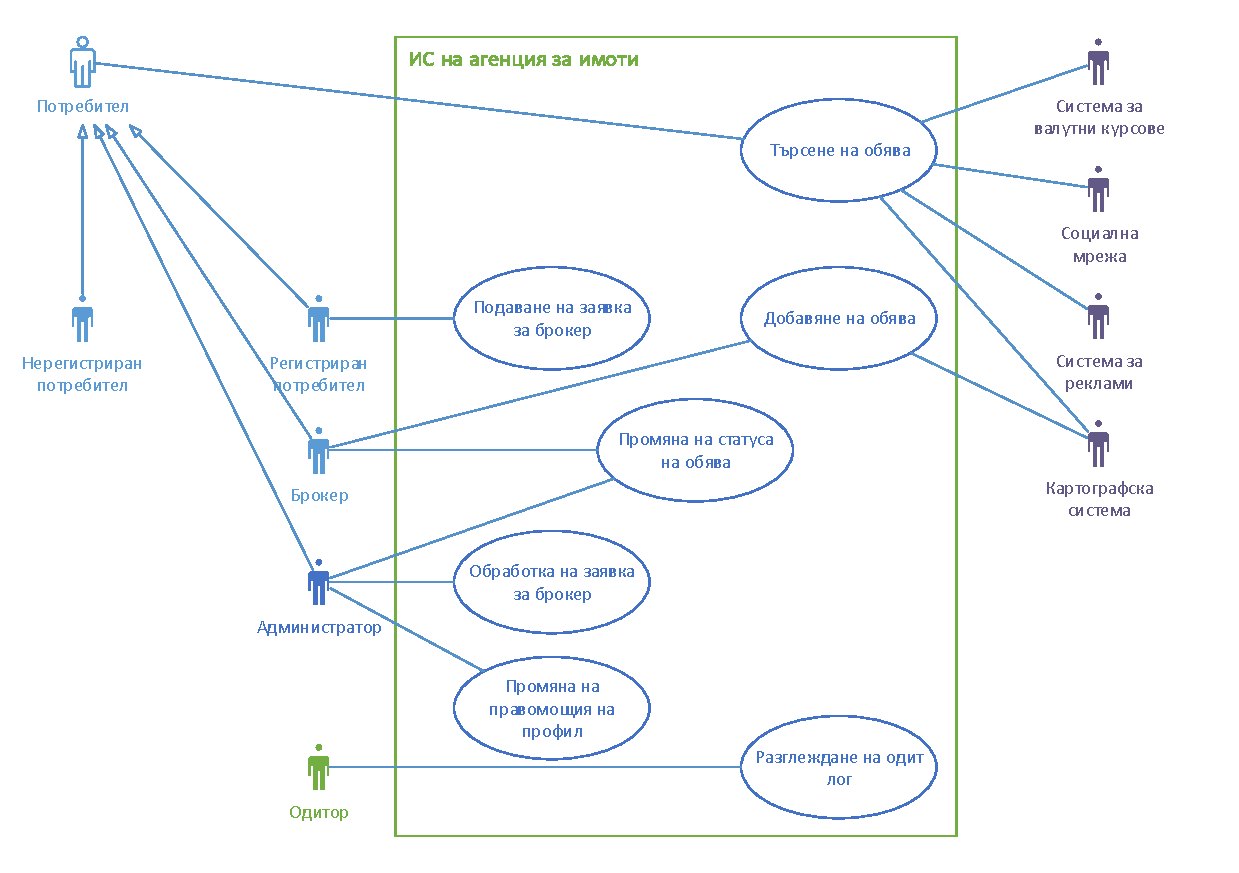
\includegraphics[scale=0.8]{use.case.model/uc1-a}
        \caption{Use case модел на потребителските случаи с приоритет A}
        \end{figure}

\clearpage

        \begin{figure}[h]
        \centering
        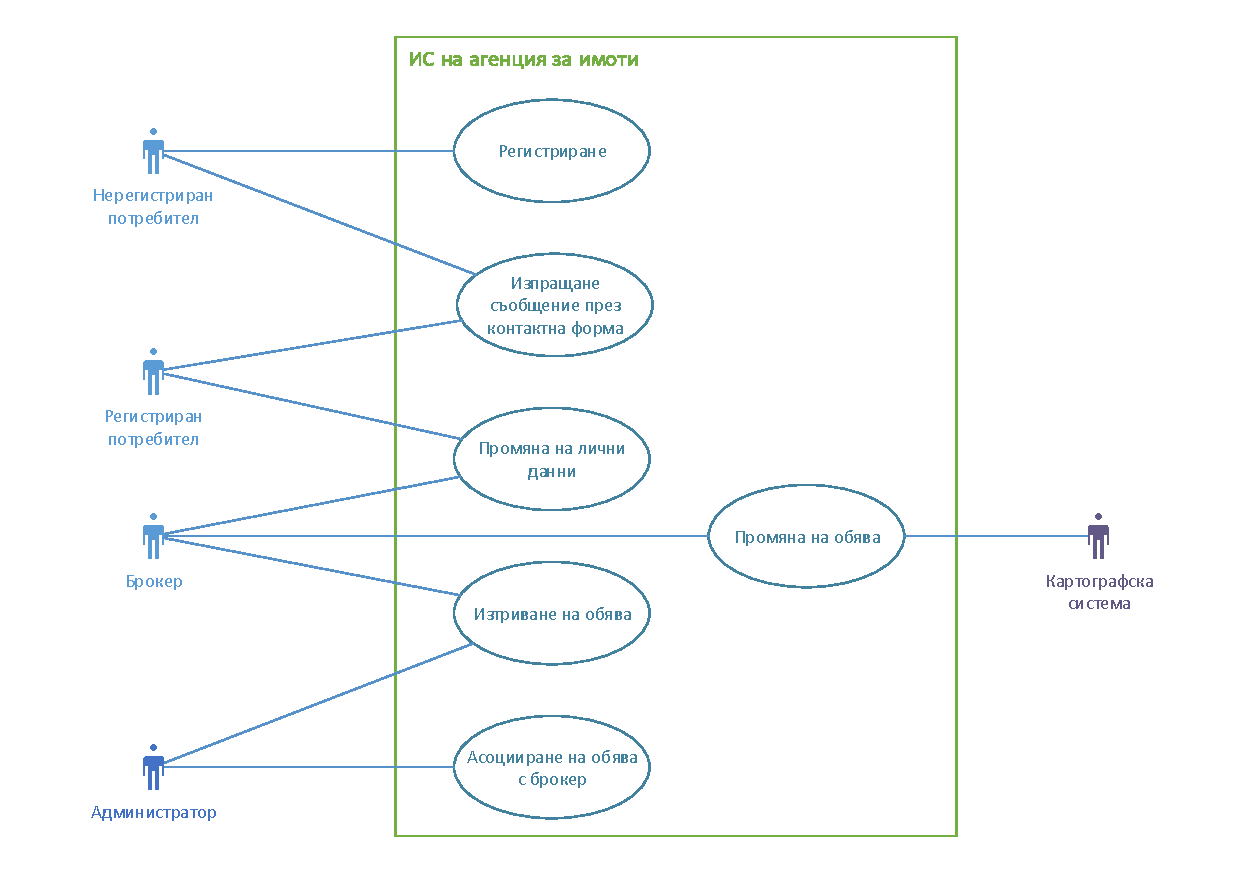
\includegraphics[scale=0.8]{use.case.model/uc1-b}
        \caption{Use case модел на потребителските случаи с приоритет B}
        \end{figure}

\clearpage

        \begin{figure}[h]
        \centering
        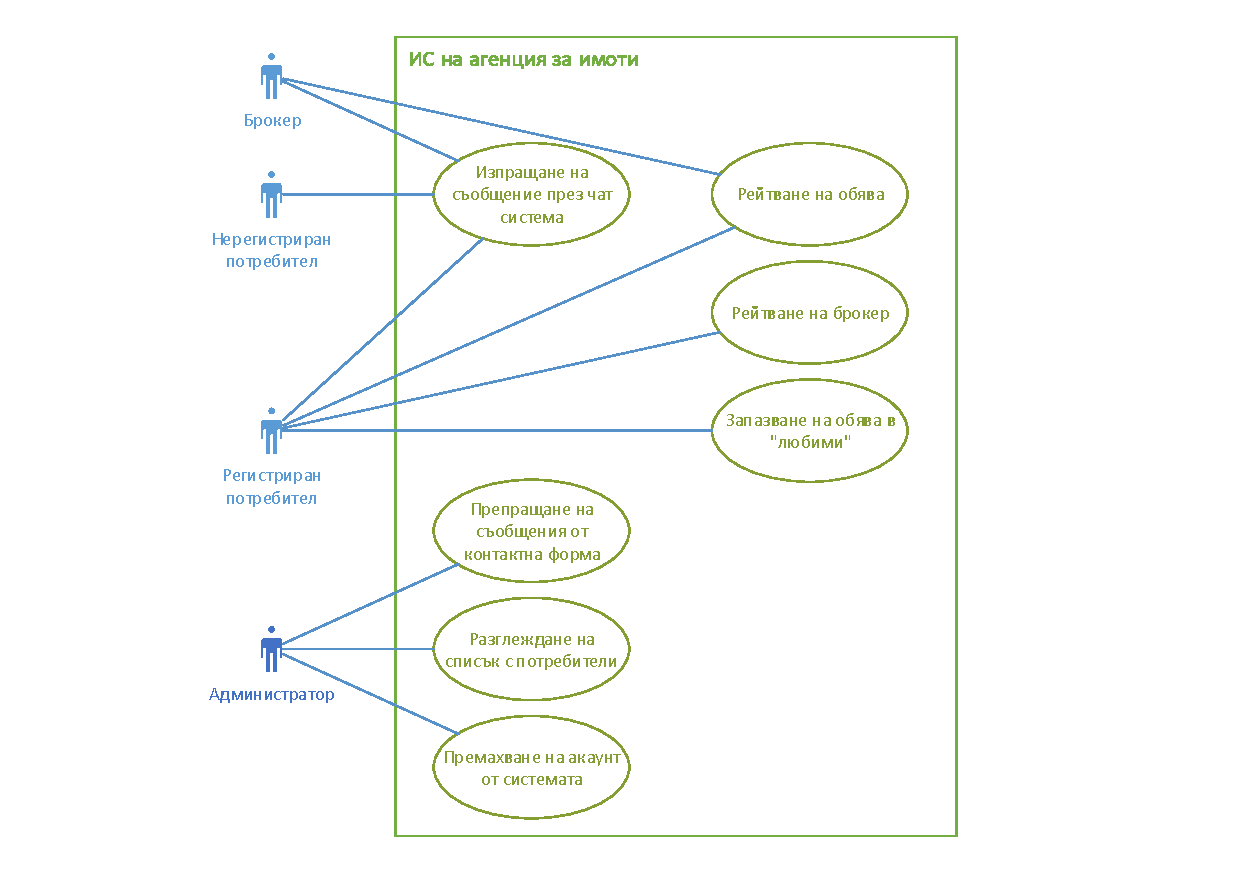
\includegraphics[scale=0.8]{use.case.model/uc1-c}
        \caption{Use case модел на потребителските случаи с приоритет C}
        \end{figure}

\section*{Списък с актьори}

\subsection{Главни}
\begin{enumerate}
\item Нерегистриран потребител
\item Регистриран потребител
\item Брокер
\item Администратор
\item Одитор
\end{enumerate}

\subsection{Второстепенни}
\begin{enumerate}
\item Система за реклами
\item Система за валутни курсове
\item Картографска система
\item Социални мрежи
\end{enumerate}


\section*{Списък на потребителските случаи} %FIXME



\section*{Шаблон за пълно описание на потребителските случаи}

\begin{usecase}
\addtitle{Use Case \emph{<номер>}}{\emph{<име на потребителският случай>}} 
\addfield{Level:}{\emph{<user-goal или subfunction>}}
\addfield{Primary Actor:}{\emph{<основен актьор>}}
\additemizedfield{Stakeholders:}{
	\item \emph{<заинтересовано лице и интереси>}
}
\additemizedfield{Preconditions:}{
	\item \emph{<предусловие>}
}
\additemizedfield{Postconditions:}{
	\item \emph{<следусловие>}
}
\addfield{Trigger:}{\emph{<условие за стартиране>}}
\addscenario{Main Success Scenario:}{
	\item \emph{<стъпка>}
	\item \emph{<стъпка>}
}
\addscenario{Extensions:}{
        \item[2.a] \emph{<Алтернативна стъпка на такава от основния сценарий>}:
                \begin{enumerate}
                \item[1.] \emph{<стъпка от алтернативния сценарий>}
                \item[2.] \emph{<стъпка от алтернативния сценарий>}                
                \end{enumerate}
        \item[5.a] \emph{<Алтернативна стъпка на такава от основния сценарий>}:
                \begin{enumerate}
                \item[1.] \emph{<стъпка от алтернативния сценарий>}
                \item[2.] \emph{<стъпка от алтернативния сценарий>}                
                \end{enumerate}
}                
\additemizedfield{Special Requirements:}{
        \item \emph{<специално изискване>}
        \item \emph{<специално изискване>}
}
\addfield{Frequency of Occurrence:}{\emph{<колко често се случва потребителският случай>}}

\end{usecase}

\section*{Пълно описание на потребителските случаи} %FIXME

\section*{Начално описание на нефункционалните изисквания}

%\subsection{Функционалност (Functionailty)}
%\begin{enumerate}
%\item Търсене на обяви - системата предлага търсене в свободен текст и филтриране на обяви
%\item Чат - системата предоставя възможност на потребителя да се свърже с брокер от агенцията чрез чат в браузера
%\item Контактна форма - системата позволява на потребителите да се свържат с брокер като му предоставят информация за обратна връзка
%\item Геолокация - системата показва на потребителите точните GPS координати на обектите в Google Maps
%\item Одит лог - системата позволява да се преглежда историята на извършените действия и данни за извършителя
%\item ВИП обяви - брокерите могат да маркират определени обяви като ВИП като така те получават приоритет в търсенето
%\item Реклами - системата е съвместима с Google Ads и показва рекламни банери
%\item Работа с различни валути - потребителите могат да изберат в каква валута да са цените измежду долар, лев и евро
%\item Пресмятане на цена - системата автоматично изчислява каква е цената на квадратен метър на даден имот
%\item Сигурност на потребителя - паролите се пазят на отделен сървър и се съхраняват чрез "salt and hash" метода
%\item Рейтинг на обяви и брокери - регистрираните потребители могат да дават рейтинг от 0 до 5 за обявите и брокерите
%\end{enumerate}

\subsection{Usability}
\begin{enumerate}
\item Снимков материал -- потребителите трябва да могат лесно да преглеждат различните налични снимки на имотите, системата трябва да поддържа поне 20 снимки на обява
\item Схема на имотите -- потребителите трябва да имат достъп до схемата на имота която показва детайлните размери на имота (стаи и т.н.)
%\item Информация за обявите -- информацията за обявите е под формата на заглавна снимка (и карта за non-mobile) и полета с текст 
\item Администраторски интерфейс -- администраторът трябва да има специален интерфейс, чрез който да вижда информация за системата и потребителите и да ги администрира
\item Брокерски интерфейс -- брокерите трябва да имат собствен интерфейс, който им помага да управляват обявите си, и им предоставя достъп до чат системата и заявките за контакт
\item Съвместимост с мобилни устройства -- интерфейсът на системата трябва да работи адекватно на различните мобилни устройства (телефони, таблети, тамагочи)
\end{enumerate}

\subsection{Reliability}
\begin{enumerate}
\item Загуба на данни -- системата не трябва да допуска загуба данни, въведени преди повече от 24 часа
\item Downtime -- системата не трябва да е в неизправност повече от 48 часа общо на година
\item Архив -- системата трябва да съхранява архивно копие на всеки 24 часа и да бъде достъпна по време на изготвянето на архивното копие. Архивни копия, по-стари от 1 месец не е задължително да се пазят.
\item Одит лог -- системата трябва да поддържа одит лог на извършените действия за последните 6 месеца, който да не може да се променя от никого
\end{enumerate}

\subsection{Performance}
\begin{enumerate}
\item Бързина на търсене -- системата трябва да намира обявите, отговарящи на дефинираните критерии за търсене за до 3 секунди
\item Бързина на зареждане на страница -- системата трябва да позволява зареждане на страница от страна на потребителите за до 1.5 секунди
\item Брой обяви -- системата трябва да може да поддържа до 10 000 обяви
\item Брой активни обяви в даден момент -- системата трябва да може да поддържа до 400 активни обяви
\item Допустим размер на снимки -- системата трябва да позволява съхранение на снимки и скици (максимум 20 броя) с индивидуален размер до 1 MB всяка.
\end{enumerate}

\subsection{Supportability}
\begin{enumerate}
\item Експлоатация -- системата трябва да е проектирана да остане в експлоатация до 10 години
%\item Логинг на данни - в одит лога ще се записват IP-адресите на на извършителите на действия и какво са извършили
\end{enumerate}

\subsection{Interface constraints}
\begin{enumerate}
\item Интерфейс -- системата трябва да предоставя web интерфейс, достъпен чрез стандартните браузъри (Chrome, Mozilla, IE/Edge, Opera, Safari), който да може да функционира адекватно и на мобилни устройства
%\item Мобилен интерфейс - интерфейс който да функционира адекватно на мобилни устройства
\end{enumerate}

\subsection{Design constraints}
\begin{enumerate}
\item Съхранение на данни -- съхранението на данни трябва да се осъществява чрез релационна база данни. Допуска се съхранение на BLOB обекти (картинки) извън СУБД.
\end{enumerate}

\subsection{Implementation constraints}
\begin{enumerate}
\item Операционна система -- системата трябва да е проектирана да работи върху GNU/Linux операционна система
\item Програмно осигуряване -- системата трябва да е базирана върху лесно достъпен в различните GNU/Linux дистрибуции free software
%\item Linux платформа - всичко което правим трябва да е съвместимо и легално в Linux
\end{enumerate}

%\subsection{Physical constraints}
%\begin{enumerate}
%\item Размери на сървъра - Сървъра ни трябва да се побере на планетата Земя (някакси)
%\end{enumerate}

\section*{Речник} %FIXME

\section*{Разпределение на времето и задачи} %FIXME
\setcounter{table}{0}

\begin{table}[h]
\centering
\caption{Време в минути за работа на всеки студент}
\label{my-label}
\begin{tabular}{|l|l|l|l|l|l|l|l|l|l|l|}
\hline
                        	& 71469 & 71473 & 71488 & 71490 & 71492 & 71508 & 71512 & 71524 & 71529 & 855240 \\ \hline
Коригиране на I-ва част		& 0     & 0     & 0     & 0		& 0     & 0     & 0   	&  0    & 0     & 0      \\ \hline
Визия						& 0     & 0     & 0     & 0		& 0     & 0     & 0   	&  0    & 0     & 0      \\ \hline
Use Case модел				& 0     & 0     & 0     & 0		& 0     & 0     & 0   	&  0    & 0     & 0      \\ \hline
Списък Актьори				& 0     & 0     & 0     & 0		& 0     & 0     & 0   	&  0    & 0     & 0      \\ \hline
Списък UC (brief)			& 0     & 0     & 0     & 0		& 0     & 0     & 0   	&  0    & 0     & 0      \\ \hline
Шаблон за UC				& 0     & 0     & 0     & 0		& 0     & 0     & 0   	&  0    & 0     & 0      \\ \hline
Fully dressed UC			& 0     & 0     & 0     & 0		& 0     & 0     & 0   	&  0    & 0     & 0      \\ \hline
Нефункционални изисквания	& 0     & 0     & 0     & 0		& 0     & 0     & 0   	&  0    & 0     & 0      \\ \hline
Речник						& 0     & 0     & 0     & 0		& 0     & 0     & 0   	&  0    & 0     & 0      \\ \hline
Review						& 0     & 0     & 0     & 0		& 0     & 0     & 0   	&  0    & 0     & 0      \\ \hline
Подготовка на доклад 2  	& 0     & 0     & 0     & 0		& 0     & 0     & 0   	&  0    & 0     & 0      \\ \hline
\textbf{Общо}           	& 0     & 0     & 0     & 0		& 0     & 0     & 0   	&  0    & 0     & 0      \\ \hline
\end{tabular}
\end{table}

\begin{table}[h]
\centering
\caption{Разпределение на работата по потребителските случаи}
\label{my-label}
\begin{tabular}{|l|l|l|}
\hline
\textbf{ф.н.} & \textbf{Име}        & \textbf{Потребителски случай}									\\ \hline
71469         & Георги Димов        & 																\\ \hline
71473         & Цветан Цветанов     & 																\\ \hline
71488         & Антон Дудов         & 																\\ \hline
71490         & Венцислав Конов     & 																\\ \hline
71492         & Александър Танков   & 																\\ \hline
71508         & Красимир Тренчев    & 																\\ \hline
71512         & Александър Велин    & 																\\ \hline
71524         & Анджелика Туджарска & 																\\ \hline
71529         & Александър Бранев   & 																\\ \hline
855240        & Мартин Стоев        & 																\\ \hline
\end{tabular}
\end{table}

\end{document}
